
\section{Café Gumbel}

Das Café Gumbel ist ein vor Jahrzehnten erstreikter Aufenthalts- und Lernraum mit Teeküche.  Das Gumbel wird von Studierenden betrieben.  Während der
Öffnungszeiten ist der Raum inklusive Küche mit Wasserkocher und Geschirr
jedem zugänglich.

Falls du gerne einen Poetry Slam, Spieleabend oder
eine andere Veranstaltung für dich und deine Kommilitonen organisieren
möchtet, frag einfach an.  Wir stellen euch gerne einen Beamer, Soundanlage,
Spielkarten (usw.) zur Verfügung.

Theresienstr., B030\\
Mo -- Fr: 8:00 -- 22:00~Uhr (meistens)\\
Kontakt: \url{gumbel@fs.lmu.de}

\skiptobottom
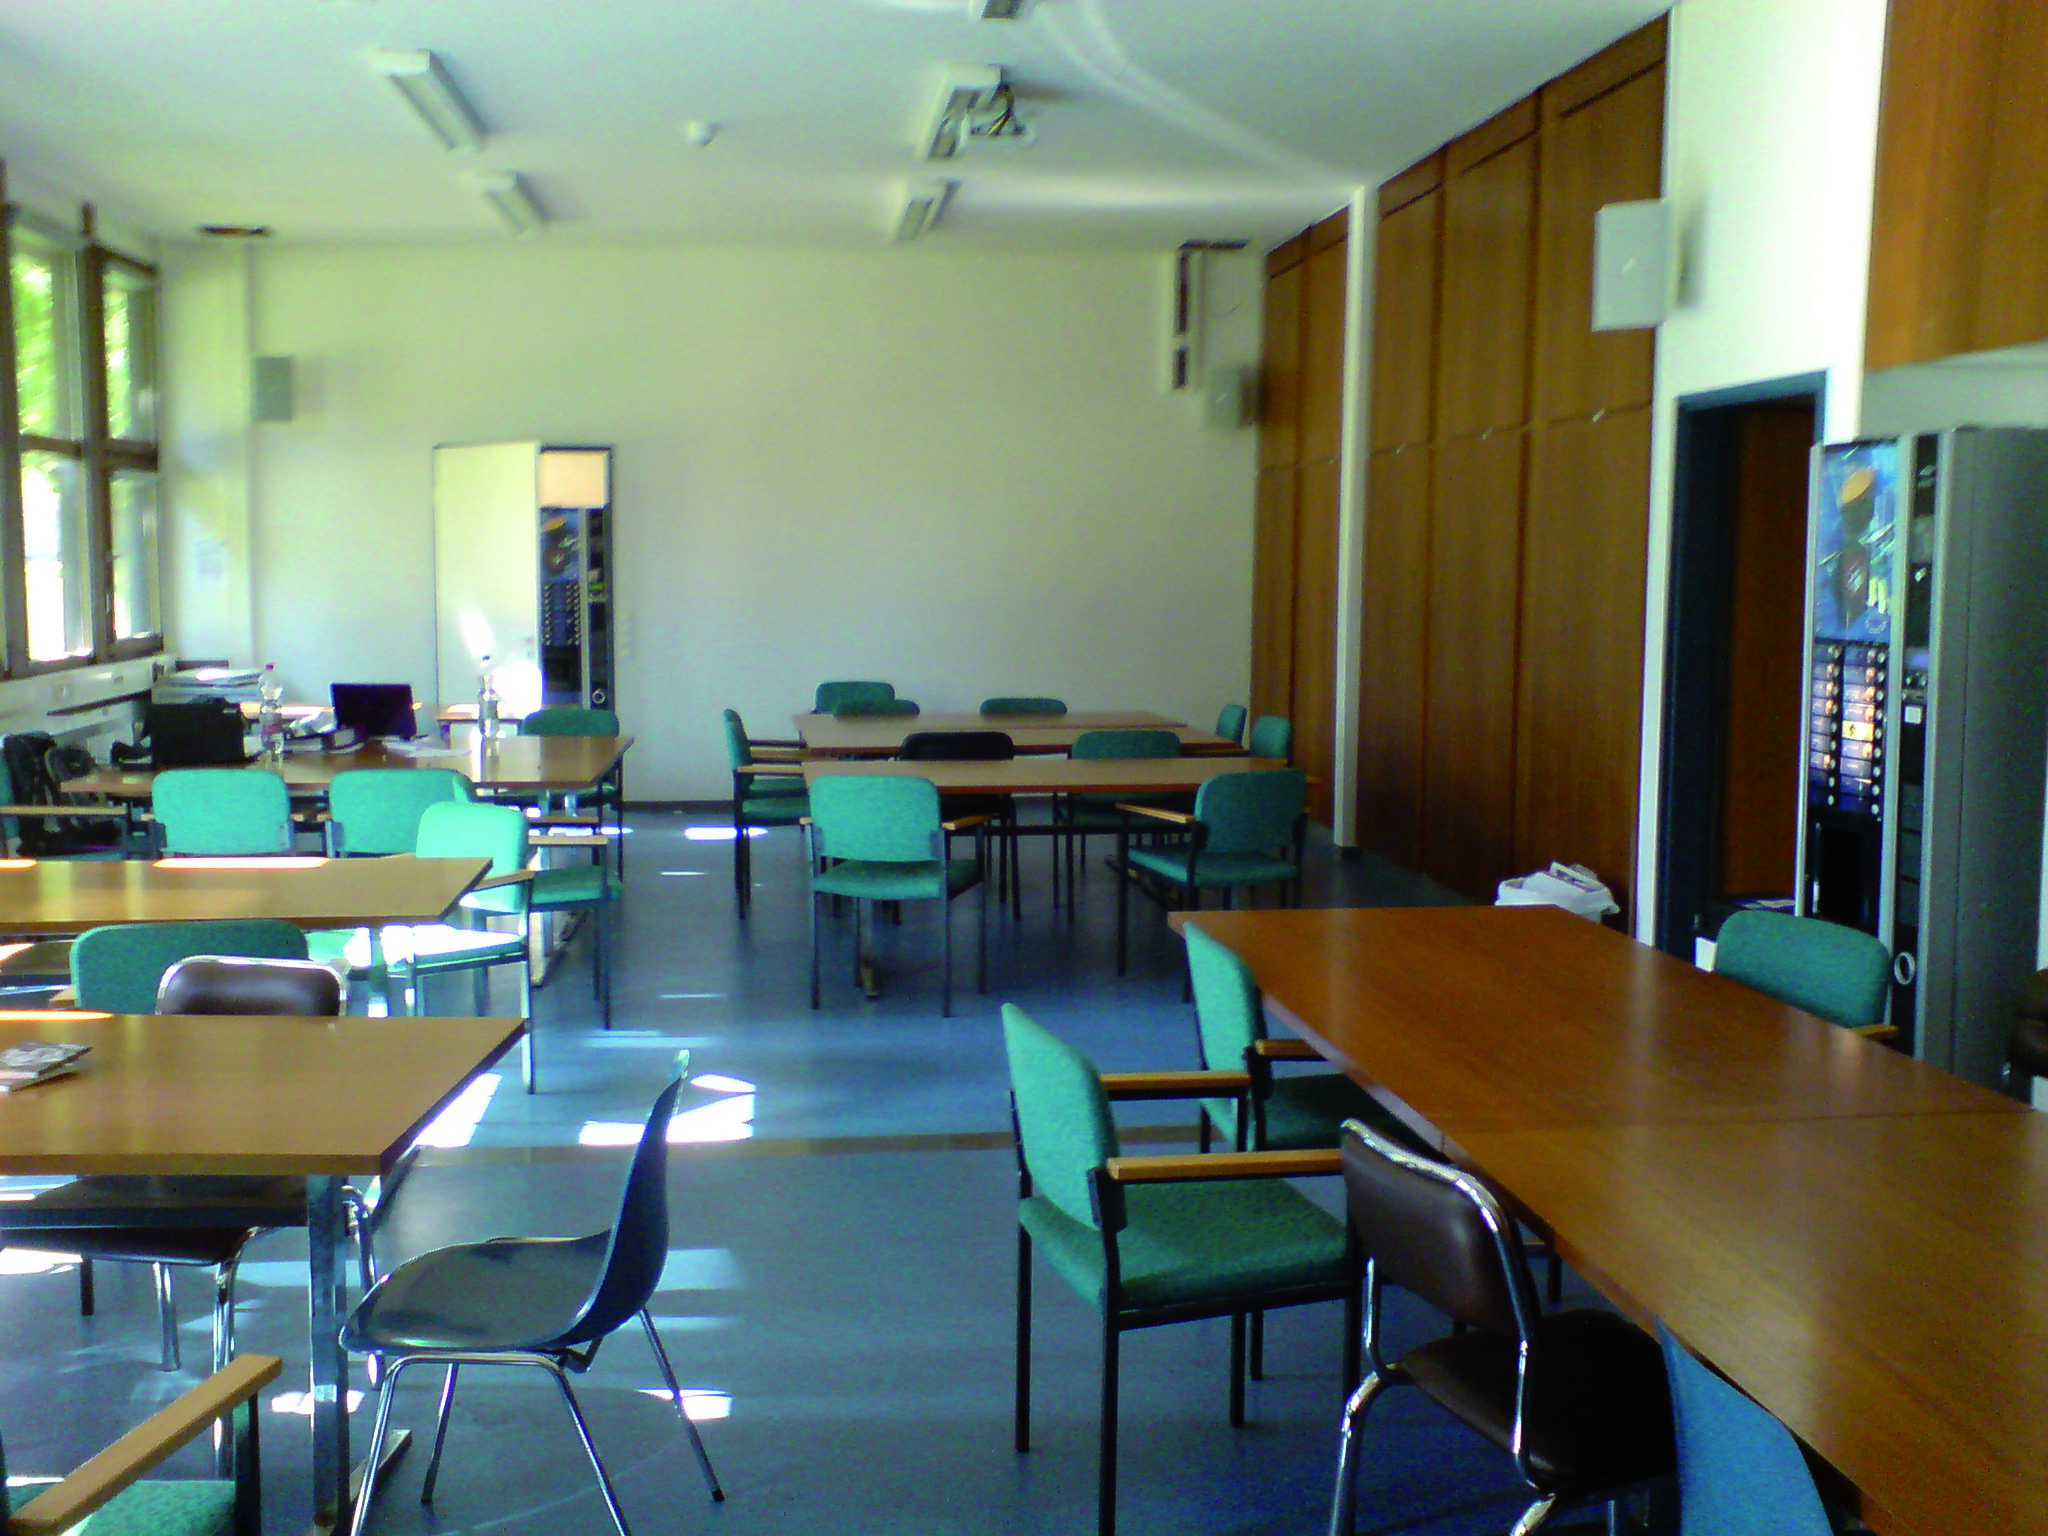
\includegraphics[width=\textwidth]{gumbel_raum_print}
